\section*{Решения и комментарии}

\subsubsection*{Сравнение чисел, версия I}% (COMPARING NUMBERS, VERSION I)

Насколько мне известно, данная задача была придумана Томом Ковером %(Tom Cover) 
в 1986 году.%
\footnote{T. Cover, ``Pick the largest number''. \emph{Open problems in communication and computation.} Springer, (1987) p. 152.}
Удивительным образом, существует стратегия, гарантирующая Виктору победу с вероятностью больше $50\%$.

\medskip

До начала игры Виктор должен обзавестись вероятностным распределением на множестве целых чисел таким, что каждому целому числу назначается положительная вероятность.
(Например, он может подбрасывать монету до первой решки.
Если выпадает чётное число $2k$ орлов, то он выбирает целое число $k$, если выпадет $2k-1$ орлов, ему нужно выбрать целое число $-k$.)

Если Виктор умён, он скроет это распределение от Паулы, но, как вы увидите позже, у Виктора всё равно будет гарантия победы, даже если Паула узнает его секрет.

После того как Паула записала свои числа, Виктор выбирает целое число из его вероятностного распределения и прибавляет к нему $\tfrac12$, полученную величину  $t$ назовём «порогом».
Например, используя распределение выше, если вышло $5$ орлов до первой решки, то его случайное целое число будет $-3$, и порог $t$ будет равен~$-2 \tfrac12$.

Когда Паула начинает игру, Виктор подбрасывает монету, чтобы решить какую руку выбрать, потом смотрит на число в этой руке.
Если число превышает $t$, он полагает, что это большее из чисел Паулы; если оно меньше, чем $t$, то считает, что оно меньшее.

А почему это работает? 
Предположим, $t$ оказывается больше, чем оба числа Паулы.
Тогда ответ Виктора будет «меньшее», независимо от того, какое число ему достанется, и, таким образом, шанс угадать равен $\tfrac12$.
Если $t$ меньше обоих чисел Паулы, Виктор, несомненно, скажет «большее», и, опять, вероятность выигрыша будет равна $\tfrac12$.

Но, \emph{с положительной вероятностью}, порог $t$ может оказаться между двумя числами Паулы, и тогда Виктор выигрывает вне зависимости от того, какую руку он выбрал.
Эта возможность, и обеспечивает вероятность выигрыша более $50\%$.\heart

Ни эта, ни какая-либо другая стратегия не даёт Виктору гарантию, что при некотором фиксированном $\varepsilon>0$ вероятность выигрыша превысит $50\%+\varepsilon$.
Умная Паула может выбрать два последовательных многозначных целых числа, и тем самым, свести преимущество Виктора к самой малости.

\subsubsection*{Сравнение чисел, версия II}% (COMPARING NUMBERS, VERSION II)

Может показаться, что возможность решать, которое число увидит Виктор, является для Паулы ничтожной компенсацией того, что не она выбирает числа.
Но, на самом деле, \emph{эта} версия игры абсолютно честная:
Паула может исключить какое-либо преимущество Виктора в игре.

У неё простая стратегия --- посмотреть на два случайных вещественных числа, затем скормить Виктору то, что ближе к~$\tfrac12$.

Это приводит Виктора к чистому угадыванию.
Чтобы это понять, предположим, что число $x$, показанное ему, лежит между $0$ и $\tfrac12$.
Тогда скрытое число равномерно распределено на множестве $[0,x]\cup [1-x, 1]$, и, таким образом, с одинаковой вероятностью будет больше или меньше $x$.
Если $x>\tfrac12$, то рассматривается множество $[0, 1-x]\cup [x, 1]$, и далее рассуждение аналогично.

Конечно, Виктор может гарантировать вероятность $\tfrac12$ при любой стратегии, игнорируя само число и подбрасывая монету, так что игра абсолютно честная.
\heart

Эта замечательная игра привлекла моё внимание в ресторане в Атланте.
За столом было много умных людей и все они оказались в тупике.
Так что, если у вас не получилось найти хорошую стратегию для Паулы, то вы оказались в хорошей компании.

\subsubsection*{Синие и красные шляпы, версия I}% (RED AND BLUE HATS, VERSION I)

Не сразу очевидно, что хоть кого-то можно спасти.
Часто первой рассматривают стратегию «большинства»;
то есть, если $n\z=10$, то каждый игрок называет цвет, который он видит на пяти или более из девяти товарищей.
Но это приведёт к десяти казням, если шляпы распределены пять на пять, и наиболее очевидная модификация этой схемы при наихудшем раскладе также закончится кровавой бойней.

\medskip

Тем не менее легко спасти $[n/2]$ игроков с помощью следующего приёма.
Игрокам надо разбиться на пары (скажем, муж и жена), каждый муж выбирает цвет шляпы жены, и каждая жена выбирает цвет, \emph{противоположный} цвету шляпы её мужа.
Очевидно, если у пары шляпы одного цвета, муж останется в живых, если нет, выживет жена.

Чтобы понять, что это наилучший возможный вариант, представим, что цвета распределяются не противником, а равномерно случайным образом (например, подкидывая монету).
Независимо от стратегии, вероятность того, что какой-либо конкретный игрок выживет, равна $\tfrac12$.
Значит, матожидание числа выживших равно $n/2$. 
Из этого следует, что \emph{минимальное} число выживших не может превысить $[n/2]$.\heart

\subsubsection*{Синие и красные шляпы, версия II}% (RED AND BLUE HATS, VERSION II)

Эту версию про красные и синие шляпы мне рассказала Гириджа Нарликар из лабораторий Белла, %(Girija Narliar of Bell Labs)
она услышала её на одной вечеринке (предыдущая версия --- мой ответ на задачу Гиринджи, хотя, несомненно, она была известна прежде).
В версии с шеренгой легко увидеть, что можно спасти $[n/2]$ игроков.
Например, игроки $n, n-2, n-4,\dots$
могут назвать цвет шляпы товарища, стоящего прямо перед ним, так что игроки $n-1, n-3,n-5,\dots$
повторяют предыдущий ответ и спасаются.

\medskip

Кажется, что вероятностное решение, как и в версии с одновременным угадыванием, должно сработать и здесь, то есть показать, что $[n/2]$ --- максимальное возможное число спасённых игроков.
Вовсе нет --- можно спасти всех игроков, кроме последнего!

Последний в шеренге игрок (несчастный бедолага!) просто говорит:
«Красная», если он видит нечётное число красных шляп впереди себя, в противном случае говорит: «Синяя».
Игрок с номером $n-1$ сможет отгадать, какого цвета на нём шляпа.
Например, если он услышал, что игрок $n$ сказал:
«Красная» и видит \emph{чётное} число красных шляп впереди себя, то он знает, что на нём красная шляпа.

Таким же образом рассуждает каждый последующий в очереди игрок.
Игрок под номером $i$ суммирует число красных шляп, которые он видит, и число услышанных «красных» ответов.
Если это нечётное число, он говорит «Красная», если чётное --- «Синяя», и угадывает правильно (если только кто-то не напортачил).

Конечно же, последнего игрока нельзя спасти, так что $n-1$ --- наилучший возможный вариант.
\heart

Стоит отметить (спасибо Джо Булеру %(Joe Buhler)
за напоминание), что даже при наличии $k$ различных цветов шляп вместо двух, только последний в шеренге игрок приносится в жертву(отправится на казнь).
Он кодирует цвета как $0, 1, 2, \dots, k-1$ и суммирует все цвета шляп, которые он видит, по модулю $k$.
Затем он объявляет цвет соответственно полученной сумме, и теперь каждый последующий игрок может определить цвет своей шляпы, вычитая из заявленного первым цвета сумму цветов, которые он видит, и цветов, названных предыдущими игроками.

Стратегия последнего игрока (при $k=10$) возможно используется вашим банком для генерирования последней цифры номера банковского счёта.

\subsubsection*{Ставка на следующую карту, версия I}% (BETTING ON THE NEXT CARD, VERSION I)

Похоже, что Виктор может добиться небольшого преимущества, дождавшись момента, когда в колоде останется больше красных карт, чем чёрных, и тогда сделать ставку.
Конечно, этого может никогда и не случиться, и если так, Виктор проигрывает.
Компенсируется ли это гораздо большей вероятностью получения малого преимущества?

В действительности это честная игра.
У Виктора не только нет способа добиться какого-либо преимущества, у него нет и возможности его потерять.
Все стратегии равно неэффективны.

Этот факт является следствием теоремы Дуба об остановке %(of the martingale stopping time theorem) 
и может быть легко доказан индукцией по числу карт каждого цвета в колоде.
Но существует другое доказательство, которое я приведу ниже, и которое, без сомнения, содержится в «Книге».\footnote{Как известно многим читателям, великий, ныне покойный, математик Пал Эрдёш часто говорил о Книге, имеющейся у Бога, в которой записаны лучшие доказательства для всех теорем.
Я представляю себе, что Эрдёш с великим удовольствием читает сейчас эту книгу, но нам придётся ещё подождать.}

Предположим, Виктор выбрал некую стратегию $S$.
Применим $S$ к несколько модифицированной версии этой задачи.
В новом варианте Виктор прерывает Паулу, как и прежде, но на этот раз он делает ставку не на \emph{следующую} карту, а на \emph{последнюю} карту в колоде.

Разумеется, в любой ситуации у последней карты точно такая же вероятность оказаться красной, как и у следующей карты в колоде.
Таким образом, стратегия $S$ имеет в новой игре такое же матожидание, как и в предыдущей.

И, конечно же, проницательный читатель уже заметил, что новый вариант игры довольно неинтересен.
Виктор выигрывает, если последняя карта --- красная, независимо от стратегии.
\heart

В книге Т. Ковера и Дж.Томаса% «Элементы теории информации»
\footnote{T. Cover and J. Thomas, \emph{Elements of Information Theory,} Wiley (1991).} 
эта игра обсуждается на основе результата статьи Т. Ковера.%
\footnote{T. Cover, ``Universal Gambling Schemes and Complexity Measures of Kolmogorov and Chaitin''. \emph{Statistics Department Technical Report \#12}, Stanford University, October 1974.}

Модифицированная версия игры %«Следующая карта --- красная»
напоминает об игре, которая много лет назад была описана --- в сатирических целях --- в журнале «Гарвардский пасквилянт».\footnote{Harvard Lampoon Vol. CLVII, No. 1, March 30, 1967, 14--15.
Номер журнала называется «Games People Play Number», и авторами рассматриваемой игры являются, по всей видимости, Д. Кенни и Д. Макклелланд.%(D.C. Kenney and D.C.K. McClelland).
}
Называлась она «Великая игра во искупление и отпущение грехов».
По правилам игроки делают ходы, бросая кубик, и двигаются по круговому полю, похожему на поле «Монополии», пока каждый из них не оказывается на клетке с надписью «Смерть».
Так кто же выигрывает?

В начале игры всем раздаётся по одной карте из «Колоды Судьбы», рубашками вверх.
В конце игры карты открываются, и те, у кого карта «Проклят», проигрывают.

\subsubsection*{Ставка на следующую карту, версия II}% (BETTING ON THE NEXT CARD, VERSION II)

Наконец-то Виктору досталась действительно хорошая игра.
Но может ли он гарантированно сыграть лучше, чем просто удвоить свои деньги, вне зависимости от того, как распределены карты?

\medskip

Для начала полезно будет подумать, какие же из стратегий Виктора будут оптимальными в смысле «матожидания».
Легко увидеть, что как только в колоде остаются карты одного цвета, Виктор должен ставить всё на каждом ходу до конца игры.
Назовём стратегию, которая следует этому правилу, «разумной».
Ясно, что каждая оптимальная стратегия является разумной.

Поразительно, но обратное также верно.
Не важно, какая у Виктора будет стратегия, матожидание будет тем же, при условии, что он будет действовать правильно, когда в колоде останутся карты одного цвета.
Чтобы увидеть это, рассмотрим вначале следующую \emph{чистую} стратегию: Виктор представляет себе какое-то конкретное фиксированное распределение красных и чёрных карт в колоде, и ставит \emph{всё, что у него есть,} согласно этому распределению \emph{на каждую карту}.

Конечно же, с такой стратегией Виктор почти всегда проигрывает, но если он выиграет, то он сможет купить весь Земной шар --- он унесёт домой $2^{52}$ долларов, то есть около 50 квадрильонов.
Поскольку существуют $\binom{52}{26}$ способов распределения цвета карт в колоде, матожидание выигрыша Виктора равно $2^{52}/\binom{52}{26} \approx 9{,}0813$.

Разумеется, эта стратегия не реалистична, но, согласно нашему определению, она «разумна», и, что особенно важно, \emph{каждая разумная стратегия является комбинацией чистых стратегий подобного типа}.
Чтобы это понять, вообразите себе, что у Виктора есть $\binom{52}{26}$ аспирантов, играющих для него, и каждый применяет свою (отличную от других) из чистых стратегий.

Мы утверждаем, что каждая разумная стратегия Виктора сводится к распределению неким образом его первоначальной суммы в 1 доллар среди этих помощников.
Если в какой-то момент его помощники ставят $x$ долларов на красную и $y$ долларов на чёрную карту, то это равносильно тому, что Виктор сам ставит $x-y$ (если $x > y$) на красную карту и $y-x$ на чёрную (при $y>x$).

Каждая разумная стратегия даёт некое распределение следующим образом.
Скажем, Виктор хочет поставить $0{,}08$ долларов на то, что первая карта будет красной.
Это означает, что его помощники, которые первую ставку делают на красное, получают $0{,}54$, в то время, как те, что ставят на чёрную, получают только $0{,}46$.
Если, выиграв, Виктор планирует поставить на следующем ходу $0{,}04$ на чёрную, он выделяет на $0{,}04$ больше помощникам со ставками «красная-чёрная», чем «красная-красная».
Продолжая таким образом, каждый помощник в итоге получит положенную ему сумму денег.

Теперь заметим, любая выпуклая комбинация стратегий с одинаковым матожиданием имеет то же матожидание.
Отсюда следует, что каждая разумная стратегия для Виктора имеет одно и то же матожидание выигрыша в $9{,}08$ (дающий ожидаемую прибыль в $8{,}08$ долларов).
В частности, все разумные стратегии оптимальны.

Но одна из этих стратегий \emph{гарантирует} $9{,}08$ долларов, а именно та, в которой ставка в 1 доллар поровну делится между помощниками.
Поскольку нельзя гарантировать больше, чем матожидание, эта стратегия является наилучшей возможной.\heart

На самом деле, данную стратегию достаточно легко реализовать (предполагая, как и раньше, что валюту США можно делить до бесконечности).
Если в колоде остаётся $b$ чёрных и $r$ красных карт, где $b\ge r$, то Виктор ставит $(b - r)/(b + r)$ от имеющейся у него на данный момент суммы на чёрную; если $r > b$, он ставит $(r - b)/(b + r)$ часть его денег на красную.

\medskip

Если изначальный доллар \emph{не} делится до бесконечности, а состоит из 100 неделимых центов, то ситуация усложняется.
В этом случае Виктор теряет около доллара.
Динамическая программа (написанная Иоаной Димитриу %(Ioana Dimitriu) 
из Калифорнийского университета в Беркли) демонстрирует, что при оптимальной игре, Виктор завершает игру с $8{,}08$ долларами.
Таблица ниже показывает, сколько у Виктора центов на каждой стадии правильно ведущейся игры.
\begin{figure}[h!]
\centering
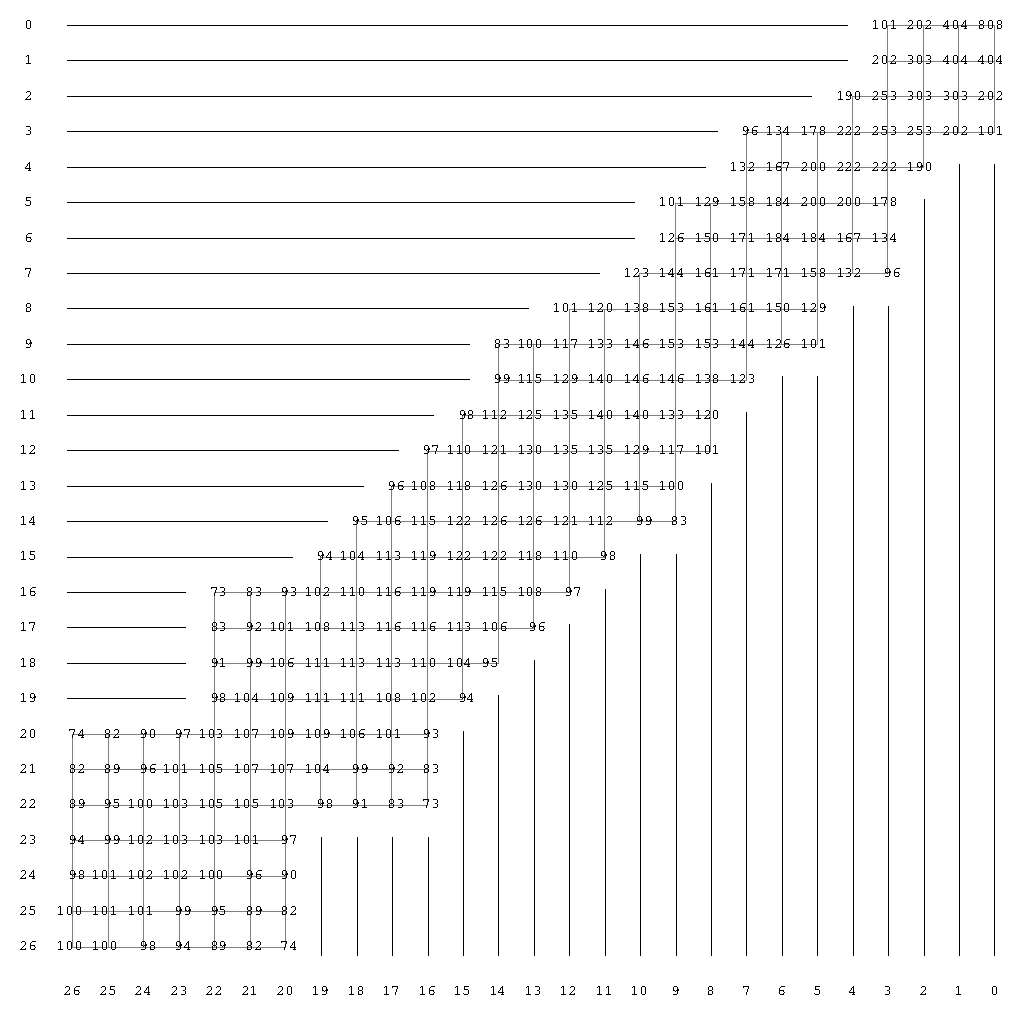
\includegraphics[scale=0.63]{Figs/Games/ioana}
\end{figure}
Например, к моменту игры, когда в колоде остаётся 12 чёрных и 10 красных карт, у Виктора должно быть $129$ центов. 
Сравнивая с числами сверху и справа, мы видим, что он должен поставить либо $11$ центов (в этом случае Паула позволяет ему выиграть) или $12$ центов (в этом случае он проиграет) на то, что следующая карта --- чёрная.

Заметьте, что в 100-центовом варианте игры Виктор делает ставки осторожней, чем в непрерывной её версии.
Если же он решит ставить каждый раз число центов, ближайшее к $(b - r)/(b + r)$ суммы его денег, то Паула разорит его ещё до того, как выйдет половина колоды!

\medskip

Я услышал эту задачу от Раса Лайонса из университета Индианы, %(Russ Lyons, of Indiana University), 
который услышал её от Ювала Переса, %(Yuval Peres), 
который услышал её от Сёрджу Харта. % (Sergiu Hart).
Сёрджу Харт не помнит, где он её услышал, но подозревает, что, скорее всего, Мартин Гарднер писал о ней десятилетия тому назад.

\subsubsection*{Гладиаторы, версия I}% (GLADIATORS, VERSION I)

Как и в первой версии «Ставки на следующую карту», все стратегии для Виктора одинаково хороши.

Чтобы это увидеть, представим себе, что сила гладиаторов --- это деньги.
Паула начинает игру с суммой в $P = p_1 + p_2 + \dots + p_m$ долларов, 
а Виктор с $V = v_1 + v_2 + \dots + v_n$.
Когда гладиатор силы $x$ побеждает гладиатора силы $y$, команда первого гладиатора получает $y$ долларов, в то время, как команда второго теряет $y$ долларов.
Общее количество денег всегда остаётся одним и тем же.
В итоге либо Паула закончит игру с $P+V$ долларами, а Виктор с $0$ долларов, либо наоборот.

Ключевое наблюдение здесь состоит в том, что каждый поединок --- честная игра.
Если Виктор выставляет гладиатора силы $x$ против гладиатора силы $y$, то ожидаемая прибыль составит 
\[\frac{x}{x+y}y + \frac{y}{x+y}(-x) =0.\]

Таким образом, весь турнир --- честная игра, из чего следует, что для Виктора ожидаемый выигрыш по окончанию игры равен той сумме, с которой он начинал, $V$.
Значит
\[q(P + V) + (1-q)(0) = V,\]
где $q$ --- вероятность того, что Виктор выигрывает.
Таким образом, $q = V/(P+V)$,
независимо от чьей-либо стратегии в турнире.
\heart

Вот ещё одно, более комбинаторное доказательство, придуманное одним из моих любимых соавторов, Грэмом Брайтвеллом, из Лондонской школы экономики. %(Graham Brightwell of London School of Economics).

Применяя приближение рациональными числами и избавляясь от знаменателей, можно предположить, что силы гладиаторов выражаются целыми числами.
Каждому гладиатору припишем $x$ шаров, если его начальная сила равнялась $x$, и расположим все шары равномерно случайным образом в вертикальном порядке.
Когда два гладиатора сражаются, тот, чей шар расположен выше, побеждает (это случается с требуемой вероятностью $x/(x+y)$), и шары проигравшего достаются победителю.

Новый набор шаров выжившего гладиатора имеет такое же однородное вероятностное распределение в начальном вертикальном порядке, как если бы он только что начал игру с полным набором шаров.
Отсюда следует, что результат каждого поединка не зависит от предыдущих событий, что и требовалось доказать.
Вне зависимости от стратегии, Виктор выигрывает тогда, и только тогда, когда самый верхний из всех шаров принадлежит ему.
Это случается с вероятностью $V/(P+V)$.

\subsubsection*{Гладиаторы, версия II}% (GLADIATORS, VERSION II)

Очевидно, что изменение правил приводит к совершенно отличным от предыдущей версии стратегическим соображениям в игре, не так ли? Нет, опять стратегии не имеют значения!

\medskip

Для этой игры, мы отберём деньги (и шары) у каждого гладиатора, и превратим его
в электрическую лампочку.

Для математика идеальная лампочка обладает следующим свойством: её время горения не имеет памяти.
Это означает, что знание того, как долго лампочка горела, абсолютно ничего нам не говорит о том, сколько времени она будет ещё гореть.

Вы, возможно, знаете, что единственное вероятностное распределение, обладающее таким свойством, --- экспоненциальное.
Если ожидаемая (средняя) продолжительность жизни лампочки равна $x$, тогда вероятность того, что она всё ещё горит в момент времени $t$, будет равна $e^{-t/x}$.
Хотя, для данной задачи нам не нужны формулы.
Необходимо только знать, что существует вероятностное распределение без памяти.

Даны две лампочки со средней продолжительностью жизни $x$ и $y$ соответственно.
Вероятность того, что первая будет гореть дольше второй, равна $x/(x+y)$.
Чтобы увидеть это, не применяя матанализ, предположим, что у нас имеется один светильник, который использует только лампочки типа «$x$», и другой, использующий только лампочки типа «$y$».
Каждый раз, когда лампочка перегорает, мы заменяем её на другую такого же типа.
Когда лампочка перегорает, вероятность того, что это $y$-лампочка, является константой, не зависящей от прошлого.
Но эта константа должна быть равной $x/(x+y)$, потому что за долгий промежуток времени $y$-лампочки и $x$-лампочки будут использованы в пропорции $x : y$.

Вернёмся в Колизей.
Представим себе, что поединок двух гладиаторов соответствует включению соответствующих им лампочек.
Они горят до тех пор, пока один из них (проигравший) не перегорает, затем победителя выключают до следующего боя.
Так как распределение не имеет памяти, сила победителя в следующем поединке не изменяется.
Замена гладиаторов лампочками может и не совсем удовлетворяет зрителей, зато является действенной моделью для сражений.

На протяжении турнира у Паулы и Виктора горит ровно по одной лампочке в любой момент времени.
Победителем является тот, чьё общее время горения (всех лампочек/гладиаторов в её/его команде) больше.
Поскольку это не имеет ничего общего с порядком, в котором включались лампочки, вероятность победы Виктора не зависит от стратегии.
(Заметим, эта вероятность --- более сложная функция от сил гладиаторов, чем в предыдущей игре.)
\heart

Игра, где сила постоянна, приводится в статье Каминского, Лакса и Нельсона.%
\footnote{K. S. Kaminsky, E. M. Luks, and P. I. Nelson, ``Strategy, Nontransitive Dominance and the Exponential Distribution''. \emph{Austral. J. Statist.}, Vol.~26, No.~2 (1984), 111--118.}
У меня есть теория, как появилась другая игра: кому-то очень понравилась эта задача и он запомнил ответ (все стратегии одинаково хороши), но не условие.
И когда он пытался воссоздать правила игры, то было совершенно естественно ввести условие наследования силы, чтобы получился мартингал.
